% Chapter 4 -- Data Mining, Multiple Testing and Backtest Overfitting
% Requires: amsmath, amssymb, booktabs, array, tabularx, graphicx, tcolorbox (breakable, skins), hyperref or url.
% Defines the callout box only if the preamble has not.
\providecolor{fenavy}{HTML}{1B2A6B}
\providecolor{feshade}{HTML}{F3F5FA}
\makeatletter
\@ifundefined{callout}{%
  \newtcolorbox{callout}{breakable, enhanced,
    colback=white, colframe=gray!70, boxrule=0.5pt, arc=1mm,
    borderline west={2.5pt}{0pt}{gray!70},
    left=8pt, right=8pt, top=4pt, bottom=4pt}%
}{}
\makeatother

\chapter{Data Mining, Multiple Testing and Backtest Overfitting}
\label{ch:04}

Every strategy you build will begin with a search. You will try ideas, adjust
settings, and compare variations until one stands out, which is how
discoveries are made in every field. The one thing to remember is that the
more you try, the higher the bar a winner must clear, and that bar can be
calculated.

A t-statistic\index{t-statistic} of about 2 is the right standard when you test a single strategy
chosen before looking at the results, for example, ``buy stocks with the
lowest price-to-book ratios,'' tested once, exactly as first stated. When the
strategy you report is the best of many you tried, the standard must rise.
Earlier chapters have already shown how it grows with the amount of searching:

\begin{itemize}
  \item \textbf{A single strategy, chosen in advance and tested once:} $t > 1.96$ (Chapter~\ref{ch:03}).
  \item \textbf{A strategy drawn from a field that has tested hundreds of others on the same data:} $t > 3$\index{t-statistic!$t>3$ hurdle} (Chapter~\ref{ch:02}).
  \item \textbf{The best of 1,000 strategies you tried yourself:} $t > 3.89$ (Chapter~\ref{ch:01}).
\end{itemize}

\textbf{Why this matters.} Whether a backtested\index{backtest} strategy is real or lucky is
more than an academic question. Many investment products, from factor funds to
the quantitative strategies run inside banks and asset managers, are built on
patterns first reported in research. Where to set the bar for evidence is therefore a
question with real money behind it, and one researchers have discussed for
decades.

Lo and MacKinlay (1990) were among the first to warn that testing ideas
suggested by earlier studies of the same data makes the evidence look stronger
than it is. The concern grew as research produced more and more
\textbf{factors}, stock characteristics such as size, value or past return
that are claimed to predict returns. Harvey, Liu and Zhu (2016) counted more
than 300 of them and suggested that a new factor should clear $t > 3$ rather
than 2, a case Harvey (2017) carried into his presidential address to the
American Finance Association. Replication\index{replication} studies added weight: Hou, Xue and
Zhang\index{q-factor model} (2020) found that about 65\% of 452 published \textbf{anomalies}\index{anomaly|textbf},
factors that standard risk models cannot explain, did not hold up once
micro-caps\index{micro-caps} were given little weight (Chapter~\ref{ch:02}).
Others see a more hopeful picture. Jensen, Kelly and Pedersen (2023), using a
Bayesian method and data from 93 countries, found that most factors do
replicate, and that strict corrections can discard real findings along with
false ones. Both sides have a point, and the claim this chapter puts on trial
sits right between them.

The claim on trial\index{claims-on-trial method} in this chapter is the one a strategy builder most needs to
be true: \textbf{with the right correction, a broad search can still find
strategies that are real.} A correction can go wrong in two ways. It can let
in a strategy that only looked good by luck, a \textbf{false discovery} (a
Type I error\index{type I error}). Or it can turn away a strategy that was genuinely real, a
\textbf{missed discovery} (a Type II error\index{type II error}). Testing the claim means measuring
both errors at once, and seeing which corrections keep the two in the best
balance.

In the lab you will do what many strategy builders do: search more than 1,000
real market-timing rules on nearly a century of U.S. data, pick the winner, and
ask whether it is skilled or just the luckiest of a thousand tries. As in a real
search, the rules come from five well-known families, and every combination of
settings counts as one rule (Table~\ref{tab:rule-universe}). A controlled
simulation, where the true strategies are known, then shows what each
correction gains and what it costs.



\begin{table}[htbp]
  \centering
  \caption{The universe of market-timing rules searched in the lab}
  \label{tab:rule-universe}
  \begin{tabular}{@{}l p{9cm} r@{}}
    \toprule
    Family & Settings varied & Rules \\
    \midrule
    Price above moving average & window 10--300 days (30 values) $\times$ band 0, 0.5, 1, 2, 5\% & 150 \\
    Moving-average crossover   & short window 5, 10, 20, 30, 50 days $\times$ long window 100, 150, 200, 250, 300 days $\times$ 5 bands & 125 \\
    Time-series momentum       & lookback 1--12 months $\times$ threshold 0, 0.5, 1, 2, 5\% & 60 \\
    Channel breakout           & window 5--250 days (8 values) $\times$ 5 bands $\times$ 5 holding periods & 200 \\
    Filter rules               & filter size 0.5--25\% (10 values) $\times$ 5 holding periods & 50 \\
    \midrule
    Subtotal                   & & 585 \\
    Both directions            & each rule run as long-or-cash and as long-or-short & $\times 2$ \\
    \midrule
    \textbf{Total}             & & \textbf{1,170} \\
    \bottomrule
  \end{tabular}

  \smallskip
  \begin{minipage}{\linewidth}
    \footnotesize
    \textit{Note:} Most of these rules are not our invention. Brock,
    Lakonishok and LeBaron (1992) found that simple moving-average and
    trading-range rules appeared to predict the Dow Jones index over about
    ninety years of data. Sullivan, Timmermann and White (1999) widened the
    search to nearly 8,000 rules, including the filter, moving-average and
    channel-breakout families used here, and asked whether the best of them
    survived once the search itself was taken into account, using the
    bootstrap Reality Check of White (2000), later refined by Hansen (2005).
    We add one modern family, time-series momentum (Moskowitz, Ooi and
    Pedersen 2012).
  \end{minipage}
\end{table}



By the end of the chapter you will be able to:

\begin{itemize}
  \item state null and alternative hypotheses\index{hypothesis testing!alternative hypothesis}, interpret a p-value\index{p-value}, explain Type I and Type II errors and power, and describe how noisy an estimated Sharpe ratio\index{Sharpe ratio} is;
  \item backtest the classic families of market-timing rules, and see how varying their settings turns a few ideas into a search over more than 1,000 strategies;
  \item explain why the 5\% significance level\index{hypothesis testing!significance level} fails when many strategies are tried, and apply the main corrections (Bonferroni\index{multiple testing!Bonferroni correction}, Holm\index{multiple testing!Holm step-down}, the false discovery rate\index{multiple testing!false discovery rate} and the $t > 3$ hurdle);
  \item judge the best of many backtests with White's Reality Check\index{White's reality check}, Hansen's test of Superior Predictive Ability\index{test of superior predictive ability}, the deflated Sharpe ratio\index{Sharpe ratio!deflated} and the probability of backtest overfitting\index{backtest overfitting!probability of (PBO)};
  \item explain why recording every trial, and deciding the test in advance, are the strongest defenses of all.
\end{itemize}

These skills are essential for building investment products, and they are
the same tools that drive the academic debates over which discoveries in finance are real.

\section{Foundations: hypothesis testing and its errors}
\label{sec:04-foundations}

\subsection{Null and alternative hypotheses}

A statistical test is a structured way of deciding whether data are strong enough to overturn a default view.

\begin{itemize}
  \item The \textbf{null hypothesis}\index{hypothesis testing!null hypothesis|textbf}, $H_0$, is the default claim the data must overturn, such as ``this strategy's true average return is zero.''
  \item The \textbf{alternative hypothesis}\index{hypothesis testing!alternative hypothesis|textbf}, $H_1$, is what we conclude if the null is rejected, such as ``the average return is positive.''
\end{itemize}

A test is \textbf{one-sided}\index{hypothesis testing!one-sided and two-sided|textbf} if only one direction counts as evidence (a positive return), and \textbf{two-sided} if either direction does.

\subsection{Test statistics and p-values}

A \textbf{test statistic}\index{hypothesis testing!test statistic|textbf} summarizes the evidence in one number; for a mean return it is the t-statistic, the estimate divided by its standard error\index{standard error}. The \textbf{p-value}\index{p-value|textbf} is the probability, computed assuming the null is true, of a statistic at least as extreme as the one observed. A small p-value says the data would be surprising if the null were true. Two common misreadings are worth naming. A p-value is \emph{not} the probability that the null is true, and it says nothing about how large or important the effect is.

\subsection{Two kinds of error}

Every test can go wrong in two ways:

\begin{center}
\small
\begin{tabularx}{0.9\linewidth}{@{}>{\raggedright\arraybackslash}p{0.18\linewidth}>{\raggedright\arraybackslash}X>{\raggedright\arraybackslash}X@{}}
\toprule
 & Null is true (no effect) & Null is false (real effect) \\
\midrule
Reject the null & \textbf{Type I error} (false discovery), probability $\alpha$ & Correct: a true discovery; probability $=$ power \\
Do not reject & Correct & \textbf{Type II error} (missed discovery), probability $\beta$ \\
\bottomrule
\end{tabularx}
\end{center}

The \textbf{significance level}\index{hypothesis testing!significance level|textbf} $\alpha$, conventionally 5\%, is the Type I error rate we accept: the chance of declaring an effect when there is none. (This $\alpha$ is unrelated to the alpha\index{alpha} of a regression.) \textbf{Power}, $1 - \beta$, is the chance of detecting an effect that is really there. Power rises with the size of the effect and the amount of data. For investment strategies, whose Sharpe ratios are modest and whose histories are short, power is often low (Chapter~\ref{ch:01}). 
Figure~\ref{fig:two-errors} shows the two errors as areas under two curves.

\providecolor{fenavy}{HTML}{1B2A6B}
\providecolor{fegray}{HTML}{4D4D4D}

\begin{figure}[htbp]
  \centering
  \begin{tikzpicture}[
    declare function={
      nullpdf(\x)=exp(-0.5*\x*\x)/sqrt(2*pi);
      altpdf(\x)=exp(-0.5*(\x-2.5)*(\x-2.5))/sqrt(2*pi);
    }]
  \begin{axis}[
    width=0.9\linewidth, height=0.45\linewidth,
    axis lines=left,
    axis line style={-stealth, thin},
    xmin=-3.5, xmax=6, ymin=0, ymax=0.5,
    xtick={0,1.96}, xticklabels={$0$,$1.96$},
    ytick=\empty,
    xlabel={$t$-statistic}, ylabel={Likelihood},
    clip=false,
    samples=200,
  ]
    % curves
    \addplot[name path=null, fegray, thick, domain=-3.5:5] {nullpdf(x)};
    \addplot[name path=alt, fenavy, thick, domain=-1:6] {altpdf(x)};
    \path[name path=axis] (axis cs:-3.5,0) -- (axis cs:6,0);

    % Type II error: real effect, but t below the critical value
    \addplot[fill=fenavy, fill opacity=0.2, draw=none]
      fill between[of=alt and axis, soft clip={domain=-1:1.96}];
    % Type I error: no effect, but t above the critical value
    \addplot[fill=gray, fill opacity=0.4, draw=none]
      fill between[of=null and axis, soft clip={domain=1.96:5}];

    % critical value
    \draw[dashed] (axis cs:1.96,0) -- (axis cs:1.96,0.47)
      node[above] {critical value};

    % curve labels
    \node[fegray] at (axis cs:-1.4,0.45) {null true: no effect};
    \node[fenavy] at (axis cs:4.6,0.45) {null false: real effect};

    % error labels
    \node[fenavy, anchor=west, align=left] (b) at (axis cs:-3.4,0.2)
      {Type II\\error ($\beta$)};
    \draw[->, fenavy] (b.east) -- (axis cs:1.2,0.09);
    \node[anchor=west, align=left] (a) at (axis cs:5.0,0.14)
      {Type I\\error ($\alpha$)};
    \draw[->] (a.west) -- (axis cs:2.35,0.025);
  \end{axis}
  \end{tikzpicture}
  \caption{The two errors of a test. The gray curve is the distribution of the
    $t$-statistic when there is no effect; the blue curve, when there is a real
    effect. A $t$-statistic beyond the critical value of 1.96 is declared
    significant. The gray area to its right is the Type I error rate; the blue
    area to its left is the Type II error rate. Moving the critical value
    shrinks one area only by enlarging the other.}
  \label{fig:two-errors}
\end{figure}


\subsection{What 5\% does and does not promise}

A 5\% test guarantees that, among tests of true null hypotheses, about one in twenty will reject by chance. It does not guarantee that one in twenty rejections is false. If most of the hypotheses tested are null, as when a researcher tries many trading rules with no real edge, most rejections can be false. This is the starting point of the chapter.

\subsection{The sampling distribution of a Sharpe ratio}

An estimated Sharpe ratio is itself a random variable: a different sample would give a different value. The range of values it could take is its \textbf{sampling distribution}\index{sampling distribution|textbf}. With $T$ periods of independent, normally distributed returns, its standard error is approximately
\begin{equation}
  \mathrm{se}(\widehat{SR}) \approx \sqrt{\frac{1 + SR^2/2}{T}}
  \label{eq:04-sese}
\end{equation}
per period, close to $1/\sqrt{T}$ when the Sharpe ratio is small. Skewness\index{skewness} and fat tails\index{fat tails} widen it (Lo 2002; Section~\ref{sec:04-deflated}). With 10 years of monthly data, $T = 120$, a monthly Sharpe ratio is uncertain by about $\pm 1/\sqrt{120} \approx \pm 0.09$, or $\pm 0.32$ in annual terms.

\textbf{Worked example.} Ten independent strategies, each with no skill, are tested at 5\%. The chance that none rejects is $0.95^{10} \approx 0.60$, so the chance of at least one ``discovery'' is about 40\%. If the researcher reports only the best one, a reader who applies the 5\% standard to it is misled.

\section{The factor zoo}
\label{sec:04-zoo}

In his 2011 presidential address to the American Finance Association, John Cochrane (2011) described the growing list of variables said to predict stock returns as a ``zoo of new factors.'' The list has kept growing. Harvey, Liu and Zhu (2016) catalogued 316 factors proposed in leading journals, most of them in the previous decade. Chen and Zimmermann's (2022) open-source replication covers more than 200 cross-sectional predictors, and McLean and Pontiff\index{anomaly!post-publication decay} (2016) studied 97 anomalies documented in academic work.

It is implausible that the cross-section of returns\index{cross-section of returns}, the differences in average return across stocks, is driven by hundreds of independent forces. Some predictors are near-duplicates of others; some are genuine; and some are what this chapter is about: results that crossed a significance threshold because many researchers tried many ideas on the same data.

The zoo is the field-level version of a problem every practitioner faces in miniature. A quantitative analyst testing variations of a trading rule, a fund family launching several strategies, a data scientist tuning a model's \textbf{hyperparameters}\index{hyperparameters|textbf} (settings chosen by the analyst rather than estimated from data, such as a window length): each runs many trials and reports the best. The statistics of that situation are the same whether the trials happen in one notebook or across a thousand journal articles.

\section{Why the 5\% level fails when many strategies are tried}
\label{sec:04-why}

A 5\% significance level means that a strategy with no skill has a 5\% chance of looking significant. That is an acceptable risk for one test. Across many tests, the risks add up.

If $N$ independent strategies with no skill are each tested at 5\%, the chance that at least one looks significant is
\begin{equation}
  P(\text{at least one false discovery}) = 1 - 0.95^N
  \label{eq:04-fwer}
\end{equation}

\begin{center}
\small
\begin{tabularx}{0.9\linewidth}{@{}>{\raggedright\arraybackslash}p{0.17\linewidth}>{\raggedright\arraybackslash}X>{\raggedright\arraybackslash}X>{\raggedright\arraybackslash}X@{}}
\toprule
Strategies tested & Chance of at least one false discovery & Expected false discoveries & Expected best t-statistic \\
\midrule
1 & 5\% & 0.05 & 0.0 \\
10 & 40\% & 0.5 & 1.5 \\
20 & 64\% & 1 & 1.9 \\
100 & 99.4\% & 5 & 2.5 \\
1,000 & effectively 100\% & 50 & 3.2 \\
\bottomrule
\end{tabularx}
\end{center}

The last column is the one Lab 1 made vivid: the expected best t-statistic rises steadily with the number of tries, roughly like $\sqrt{2 \ln N}$. With 20 tries, the best is expected to sit right at the conventional threshold; with 1,000, comfortably above it (Figure~\ref{fig:04-hurdles}). 


\providecolor{fenavy}{HTML}{1B2A6B}
\providecolor{fegray}{HTML}{4D4D4D}

\begin{figure}[htbp]
  \centering
  \begin{tikzpicture}
  \begin{semilogxaxis}[
    width=0.85\linewidth, height=0.5\linewidth,
    axis lines=left,
    axis line style={-stealth, thin},
    xmin=1, xmax=10000, ymin=0, ymax=5,
    xtick={1,10,100,1000,10000},
    xticklabels={1,10,100,{1,000},{10,000}},
    ytick={0,1,1.96,3,4,5},
    yticklabels={0,1,1.96,3,4,5},
    xlabel={Number of strategies tried, $N$},
    ylabel={$t$-statistic},
    clip=false,
  ]
    % Expected t-statistic of the best of N strategies with no skill
    \addplot[fenavy, very thick] coordinates {
      (1,0.000) (2,0.564) (3,0.846) (4,1.029) (5,1.163) (6,1.267) (8,1.424)
      (10,1.539) (13,1.668) (16,1.766) (20,1.867) (25,1.965) (32,2.070)
      (40,2.161) (50,2.249) (63,2.338) (79,2.422) (100,2.508) (126,2.589)
      (158,2.667) (200,2.746) (251,2.820) (316,2.894) (398,2.967) (501,3.037)
      (631,3.107) (794,3.175) (1000,3.241) (1259,3.307) (1585,3.371)
      (1995,3.435) (2512,3.497) (3162,3.558) (3981,3.619) (5012,3.678)
      (6310,3.737) (7943,3.795) (10000,3.852)};

    % Bonferroni hurdle, 5% two-sided: t = Phi^{-1}(1 - 0.025/N)
    \addplot[fegray, thick, dashed] coordinates {
      (1,1.960) (2,2.241) (3,2.394) (4,2.498) (5,2.576) (6,2.638) (8,2.734)
      (10,2.807) (13,2.891) (16,2.955) (20,3.023) (25,3.090) (32,3.163)
      (40,3.227) (50,3.291) (63,3.355) (79,3.417) (100,3.481) (126,3.542)
      (158,3.601) (200,3.662) (251,3.720) (316,3.778) (398,3.835) (501,3.891)
      (631,3.947) (794,4.001) (1000,4.056) (1259,4.109) (1585,4.162)
      (1995,4.214) (2512,4.266) (3162,4.317) (3981,4.368) (5012,4.418)
      (6310,4.467) (7943,4.516) (10000,4.565)};

    % Fixed hurdles
    \addplot[fegray, thin, domain=1:10000] {1.96};
    \addplot[black, thin, densely dotted, domain=1:10000] {3};

    % Crossing of 1.96 at about 25 tries
    \draw[fenavy, densely dashed, thin] (axis cs:25,0) -- (axis cs:25,1.965);
    \fill[fenavy] (axis cs:25,1.965) circle (1.6pt);
    \node[fenavy, anchor=north west, align=left, font=\small]
      at (axis cs:27,1.85) {crosses 1.96\\at $N \approx 25$};

    % Labels
    \node[fenavy, anchor=north west, font=\small] at (axis cs:300,2.7)
      {best of $N$, no skill};
    \node[fegray, anchor=south, font=\small, rotate=9] at (axis cs:1500,4.22)
      {Bonferroni hurdle};
    \node[fegray, anchor=north east, font=\small] at (axis cs:10000,1.92)
      {usual hurdle, $t = 1.96$};
    \node[anchor=south west, font=\small] at (axis cs:1.1,3.02)
      {$t > 3$ hurdle};
  \end{semilogxaxis}
  \end{tikzpicture}
  \caption{Why the hurdle must rise with the search. The blue curve is the
    $t$-statistic the best of $N$ strategies with no skill is expected to show.
    It crosses the usual hurdle of 1.96 at about 25 tries. The Bonferroni
    hurdle (Section~\ref{sec:04-corrections}) rises with $N$ and stays above
    the curve; the fixed $t > 3$ hurdle of Harvey, Liu and Zhu is a simple
    compromise.}
  \label{fig:04-hurdles}
\end{figure}


\textbf{Two kinds of error rate.} Statisticians distinguish two goals when many hypotheses are tested:

\begin{itemize}
  \item The \textbf{family-wise error rate}\index{multiple testing!family-wise error rate|textbf} (FWER) is the chance of making even one false discovery. Controlling it is strict and appropriate when a single false claim is costly, for example when one strategy will receive all the capital.
  \item The \textbf{false discovery rate}\index{multiple testing!false discovery rate|textbf} (FDR) is the expected share of false discoveries among all discoveries. Controlling it at 5\% means accepting that about one in twenty claimed findings will be false. It is appropriate when many findings are reported and some errors are tolerable, as in screening a large set of candidate factors.
\end{itemize}

\textbf{Hidden trials.} The number of tests is often far larger than it appears. Each parameter setting tried, each sample period considered, each variable definition tested and each model abandoned is a trial. A published result may report one test while resting on hundreds. Correlated trials, such as the same rule with slightly different windows, count for less than independent ones, but they still count.

\section{Corrections: Bonferroni, Holm, false discovery rate, $t > 3$}
\label{sec:04-corrections}

Each correction raises the bar for significance as the number of tests grows. They differ in which error rate they control and in how much power they sacrifice. Suppose $N$ strategies have been tested and their p-values sorted from smallest, $p_{(1)}$, to largest, $p_{(N)}$.

\begin{center}
\small
\begin{tabularx}{0.9\linewidth}{@{}>{\raggedright\arraybackslash}p{0.18\linewidth}>{\raggedright\arraybackslash}X>{\raggedright\arraybackslash}p{0.21\linewidth}>{\raggedright\arraybackslash}p{0.19\linewidth}@{}}
\toprule
Method & Rule & Controls & Strictness \\
\midrule
Bonferroni & Reject if $p \le \alpha/N$ & FWER under any dependence & Strictest; loses the most power \\
Holm (1979) & Step down: reject $p_{(k)}$ while $p_{(k)} \le \alpha/(N - k + 1)$ & FWER under any dependence & Never less powerful than Bonferroni \\
Benjamini--Hochberg (1995) & Find the largest $k$ with $p_{(k)} \le k\alpha/N$; reject all up to $k$ & FDR, for independent or positively dependent tests & Much more powerful when many effects are real \\
Benjamini--Yekutieli (2001) & As BH, with $\alpha$ divided by $\sum_{i=1}^{N} 1/i$ & FDR under any dependence & Between BH and Bonferroni \\
Fixed $t > 3$ (Harvey, Liu and Zhu 2016) & Reject if $t > 3$ & Approximates a correction for the field's history of testing & Simple rule of thumb \\
\bottomrule
\end{tabularx}
\end{center}

A \textbf{step-down} procedure such as Holm's works through the sorted p-values from the smallest, applying a slightly looser bar at each step, and stops at the first one that fails. With 1,000 tests at $\alpha = 5\%$, Bonferroni requires $p \le 0.00005$, a one-sided t-statistic of about 3.9. Benjamini--Hochberg's threshold depends on how many effects are real: when there are many, it can be close to the usual 1.96 for the strongest results.

\textbf{Choosing a correction.} None is right for every purpose. Bonferroni and Holm suit the decision to fund a single strategy, where one false positive is expensive. FDR methods suit screening, where the goal is a short list that is mostly right. The $t > 3$ hurdle is a practical summary for readers of published research: Harvey, Liu and Zhu argued that, given the number of factors already tested, a new factor should clear about $t = 3$ to be taken seriously.

\textbf{The cost of strictness.} Corrections reduce false discoveries by also rejecting some true ones. Harvey and Liu (2020) emphasized this trade-off: an investor who demands $t > 3$ everywhere will miss real but modest effects. The lab's simulation measures both sides, false discoveries and missed discoveries, for every method.

\section{Backtest overfitting and the deflated Sharpe ratio}
\label{sec:04-deflated}

Multiple-testing\index{multiple testing} corrections work on p-values. Practitioners usually judge strategies by their Sharpe ratios, and Bailey and L\'opez de Prado developed a correction expressed in those terms. A backtest is \textbf{overfit}\index{overfitting|textbf} when its rules have been tuned so closely to the noise in past data that its performance there says little about the future.

\textbf{The probabilistic Sharpe ratio.} Bailey and L\'opez de Prado (2012) first asked: given an estimated Sharpe ratio $\widehat{SR}$ from $T$ observations, what is the probability that the true Sharpe ratio exceeds a benchmark $SR^*$? Allowing for the skewness $\gamma_3$ and kurtosis\index{kurtosis} $\gamma_4$ of returns, it is approximately
\begin{equation}
  \mathrm{PSR}(SR^*) = \Phi\!\left(\frac{(\widehat{SR} - SR^*)\sqrt{T-1}}{\sqrt{1 - \gamma_3\,\widehat{SR} + \frac{\gamma_4 - 1}{4}\,\widehat{SR}^2}}\right)
  \label{eq:04-psr}
\end{equation}
where $\Phi$ is the standard normal distribution\index{distribution!normal} function, which turns a number of standard errors into a probability, and Sharpe ratios are measured per period, not annualized. Negative skewness and fat tails, both common in strategy returns, widen the uncertainty.

\textbf{The deflated Sharpe ratio.}\index{Sharpe ratio!deflated|textbf} Bailey and L\'opez de Prado (2014) then replaced the benchmark $SR^*$ with the Sharpe ratio one would expect from the best of $N$ trials if none had any skill. With $V$ the variance\index{variance} of the estimated Sharpe ratios across the trials, that expected maximum is approximately
\begin{equation}
  SR_0 = \sqrt{V}\left((1-\gamma)\,\Phi^{-1}\!\left(1 - \tfrac{1}{N}\right) + \gamma\,\Phi^{-1}\!\left(1 - \tfrac{1}{N e}\right)\right)
  \label{eq:04-sr0}
\end{equation}
where $\Phi^{-1}$ is the inverse of $\Phi$, $e \approx 2.718$, and $\gamma \approx 0.5772$ is the Euler--Mascheroni constant, a number that appears in the mathematics of maxima. The \textbf{deflated Sharpe ratio} is the PSR with $SR^* = SR_0$: the probability that the selected strategy's true Sharpe ratio is above what luck alone would deliver from $N$ tries. A value above 0.95 is the analogue of significance at 5\%.

\textbf{What $N$ should be.} The deflated Sharpe ratio requires an honest count of trials. When trials are highly correlated, such as one rule with many nearby window lengths, the \textbf{effective number of trials}\index{multiple testing!effective number of trials|textbf}, the number of truly independent bets, is smaller than the raw count. Bailey and L\'opez de Prado suggest clustering the trials (L\'opez de Prado 2019); the lab uses a simpler approximation from the correlation\index{correlation} structure of the strategies' returns and reports the result under both counts.

\textbf{Minimum backtest length.} A related result in Bailey, Borwein, L\'opez de Prado and Zhu (2014) turns the logic around: for a given number of trials, there is a minimum backtest length below which a Sharpe ratio of a given size is no evidence at all. With only a few years of data, trying even a few dozen configurations can be enough to produce an impressive in-sample\index{in-sample versus out-of-sample} Sharpe ratio from pure noise.

\section{The probability of backtest overfitting and combinatorial cross-validation}
\label{sec:04-pbo}

The deflated Sharpe ratio asks whether the best strategy is better than luck. A different question is how often the process of choosing the best \textbf{in-sample}\index{in-sample versus out-of-sample|textbf} strategy, the best on the data used to choose it, picks one that does worse than average \textbf{out of sample}, on data it has not seen. Bailey, Borwein, L\'opez de Prado and Zhu (2017) called this the \textbf{probability of backtest overfitting}\index{backtest overfitting!probability of (PBO)|textbf} (PBO) and proposed a way to estimate it.

\textbf{Combinatorially symmetric cross-validation (CSCV).}\index{combinatorially symmetric cross-validation|textbf} \textbf{Cross-validation}\index{cross-validation|textbf} means repeatedly splitting data into a part used to choose a model and a part used to check it. CSCV does this in every possible way, using the full history of every strategy tried (Figure~\ref{fig:04-cscv}):

\begin{enumerate}
  \item Split the sample into $S$ blocks of equal length, for example $S = 16$.
  \item Form every way of choosing half the blocks as a training set\index{training, validation and test sets}; the other half is the test set. With 16 blocks there are 12,870 such splits.
  \item For each split, find the strategy with the best Sharpe ratio in the training set and record its rank among all strategies in the test set, as a relative rank $\omega$ between 0 and 1.
  \item Convert each rank to a \textbf{logit}\index{regression!logit|textbf}, $\lambda = \ln(\omega / (1 - \omega))$, a transformation that is zero at the median rank, negative below it and positive above it. A negative logit means the in-sample winner ranked below the median out of sample.
  \item The PBO is the share of splits with a negative logit.
\end{enumerate}

\providecolor{fenavy}{HTML}{1B2A6B}

\begin{figure}[htbp]
  \centering
  \begin{tikzpicture}[
    x=0.44cm, y=0.62cm,
    blk/.style={minimum width=0.40cm, minimum height=0.40cm, inner sep=0pt},
    train/.style={blk, fill=fenavy},
    test/.style={blk, fill=gray!25},
    lab/.style={anchor=east, font=\small},
  ]
    % Legend
    \node[train] at (1,1.6) {};
    \node[anchor=west, font=\small] at (1.4,1.6) {training half};
    \node[test] at (8,1.6) {};
    \node[anchor=west, font=\small] at (8.4,1.6) {test half};

    % Block numbers
    \foreach \i in {1,...,16} {
      \node[font=\scriptsize, text=gray] at (\i,0.75) {\i};
    }

    % Example splits: 1 = training block, 0 = test block
    \foreach \row/\pattern in {
        1/{1,1,0,1,0,0,1,0,1,1,0,0,1,0,1,0},
        2/{0,1,1,0,1,1,0,0,1,0,0,1,0,1,1,0},
        3/{1,0,0,1,1,0,1,1,0,0,1,0,1,1,0,0}} {
      \node[lab] at (0,-\row+1) {Split \row};
      \foreach \b [count=\i] in \pattern {
        \ifnum\b=1
          \node[train] at (\i,-\row+1) {};
        \else
          \node[test]  at (\i,-\row+1) {};
        \fi
      }
    }
    \node[lab] at (0,-3) {\dots};
    \node[font=\small] at (8.5,-3) {12,870 splits in all};

    % What happens in each split (no fixed width, so lines never wrap)
    \node[anchor=north west, font=\small, inner sep=0pt] at (17.2,1.95)
      {\begin{tabular}{@{}l@{~}l@{}}
         \multicolumn{2}{@{}l}{In each split:} \\
         1. & pick the best strategy \\
            & on the training half \\
         2. & find its rank on \\
            & the test half \\
         3. & below the median? \\
            & count as overfit
       \end{tabular}};

    % PBO
    \node[anchor=west, font=\small] at (-2.6,-4.5)
      {PBO $=$ share of splits in which the winner falls below the median};
  \end{tikzpicture}
  \caption{Combinatorially symmetric cross-validation. The sample is cut into
    16 blocks. Each split assigns eight blocks to training and eight to
    testing; every one of the 12,870 possible splits is used. The probability
    of backtest overfitting is the share of splits in which the training
    winner ranks below the median in testing.}
  \label{fig:04-cscv}
\end{figure}


%\begin{figure}[htbp]
%\centering
%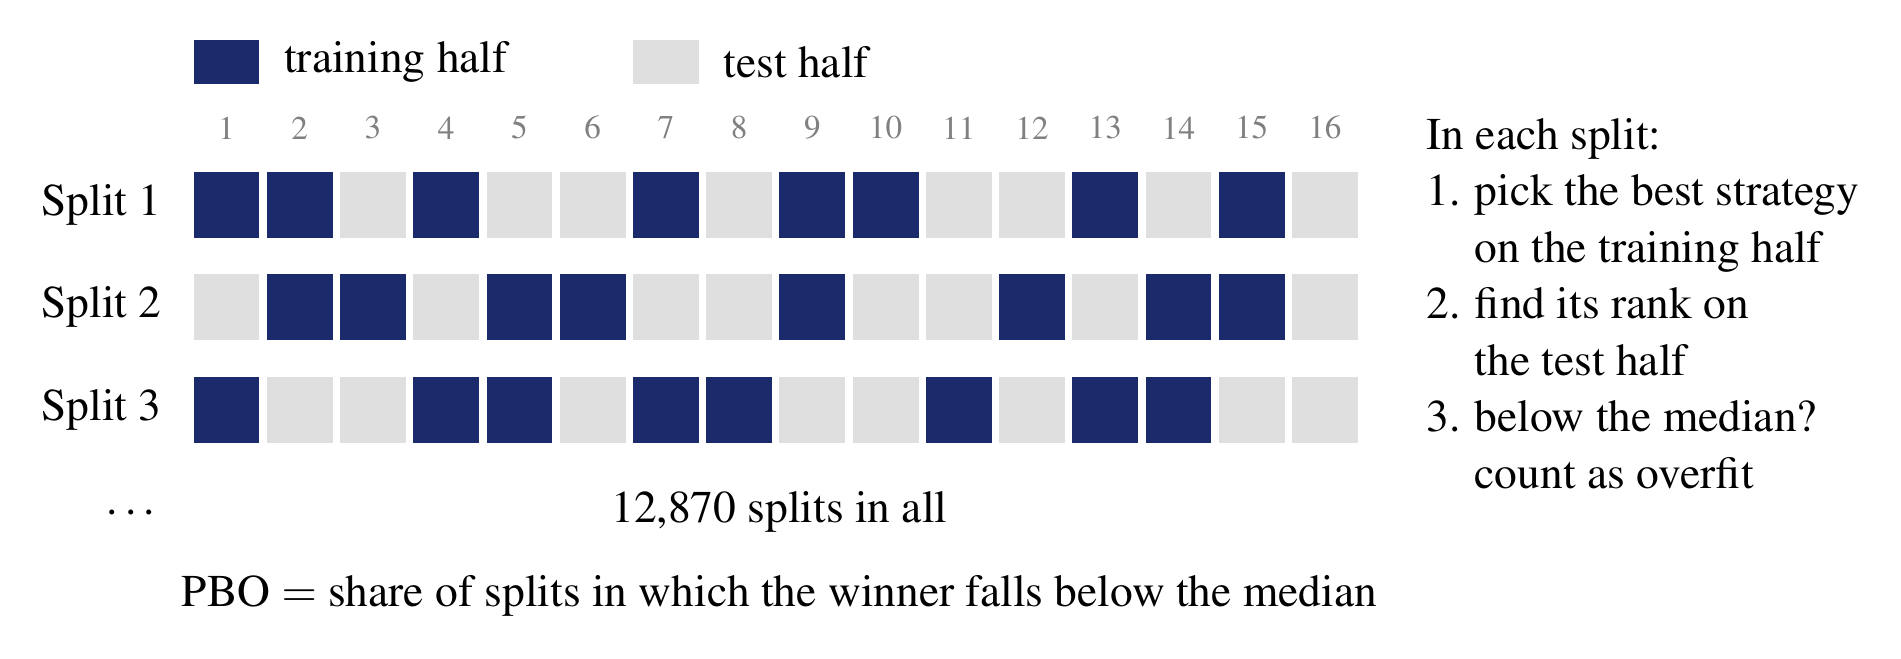
\includegraphics[width=0.9\linewidth]{images/fig04-3-cscv.png}
%\caption{Combinatorially symmetric cross-validation. The sample is cut into 16 blocks. Each split assigns eight blocks to training and eight to testing; every one of the 12,870 possible splits is used. The probability of backtest overfitting is the share of splits in which the training winner ranks below the median in testing.}
%\label{fig:04-cscv}
%\end{figure}

A PBO near 0 means the selection process reliably picks strategies that remain above average; a PBO near 0.5 means in-sample performance carries no information about out-of-sample rank; above 0.5, selection actively picks losers, a sign that the search rewards fitting noise.

CSCV has two advantages over a single train--test split. It uses every observation for both training and testing, and it produces a distribution rather than a single outcome, so one lucky or unlucky split cannot decide the verdict. Its main limitation is that blocks are treated as interchangeable, which ignores the order of time; the lab therefore also reports a conventional chronological out-of-sample test.

\section{Bootstrap reality checks and pre-registration}
\label{sec:04-reality}

\textbf{Reality checks.}\index{White's reality check|textbf} White (2000) proposed testing whether the best of many strategies beats a benchmark, using a bootstrap\index{bootstrap} (Section~\ref{sec:03-bootstrap}) that resamples all strategies' returns together and so respects their correlations. Hansen (2005) refined the test, as the superior predictive ability (SPA) test, to make it less sensitive to poor strategies included in the comparison. These tests answer the same question as the deflated Sharpe ratio, but without its distributional approximations.

\begin{callout}
\textbf{What Failed: a century of technical trading rules.} Brock, Lakonishok and LeBaron (1992) found that simple moving-average and trading-range rules applied to the Dow Jones index from 1897 to 1986 produced significant profits. Sullivan, Timmermann and White (1999) re-examined them against a universe of several thousand related rules, using White's reality check to account for the search. The best rule still looked significant in the original sample, but its superior performance did not carry over to the decade that followed. A result that survives a search can still fail the test that matters most: new data.
\end{callout}

\textbf{Pre-registration.}\index{pre-registration|textbf} Every correction in this chapter depends on knowing how many trials were run. The surest way to know is to decide in advance. \textbf{Pre-registration} means writing down, before looking at the test data, the hypothesis, the data, the sample period, the strategy's exact rules and the criteria for success, and then reporting the result whatever it is. It is standard in clinical trials and increasingly common in economics. Chapter~\ref{ch:25} shows how to write one.

For practitioners without a formal registry, three habits come close:

\begin{enumerate}
  \item \textbf{Keep a trial log.} Record every configuration tested, including those abandoned. It is the input every correction needs.
  \item \textbf{Hold out data you never look at} until the strategy's design is final, and use it once.
  \item \textbf{Prefer economic reasons stated before the test.} A rule motivated by a mechanism is less likely to be an artifact than one found by search and explained afterward.
\end{enumerate}

\section{Lab 4: The best of a thousand rules}
\label{sec:04-lab}

\begin{callout}
\textbf{Lab 4 at a glance.} \emph{Claim on trial:} with the right correction, a broad search can still find strategies that are real. \emph{Data:} monthly U.S. market and Treasury bill returns, from the Kenneth R. French Data Library\index{Kenneth French data library} (Fama/French 3 Factors). \emph{Run time:} under a minute. \emph{Code:} repository folder \texttt{ch04-overfitting/}, with a guided notebook.
\end{callout}

The lab recreates, in miniature, the situation behind the factor zoo\index{factor zoo}. It searches a large family of market-timing rules for the best backtest, then asks whether the winner is a discovery.

\textbf{The rules.} Every rule is either fully in the U.S. stock market or in Treasury bills, and decides at the end of each month for the next. There are 473 rules:

\begin{itemize}
  \item prices above moving averages\index{moving average} of 2 to 24 months, with and without bands;
  \item crossovers of fast and slow moving averages;
  \item \textbf{time-series momentum}\index{momentum!time-series|textbf} over 1 to 24 months: holding the market when its own past return is positive;
  \item seasonal rules that leave the market for some months of the year;
  \item a volatility\index{volatility} filter.
\end{itemize}

Each also appears in a \textbf{contrarian}\index{contrarian strategy|textbf} version, which does the opposite, for 946 rules in all. Nothing here is exotic. Every rule is the kind of thing a curious analyst might try on a Sunday afternoon.

\textbf{The skill measure.} A rule that is in the market most of the time will earn most of the equity premium\index{equity premium}, which is not skill (Section~\ref{sec:01-foundations}). The lab therefore scores each rule by its \textbf{hedged return}\index{return!hedged|textbf}: the rule's excess return\index{return!excess} minus its beta\index{beta} times the market's. A rule that always holds the market scores exactly zero. The Sharpe ratio of the hedged return is the rule's \textbf{appraisal ratio}\index{appraisal ratio|textbf}, and its t-statistic is the t-statistic of the rule's alpha.

\textbf{Part A: the search.} The rules are backtested on the first half of the sample, roughly 1929 to 1977. The lab reports how many rules clear each decision rule from Section~\ref{sec:04-corrections}, the best rule's deflated Sharpe ratio with both the raw and the effective number of trials, and then what every rule did in the second half, which played no part in the search.

The effective count needs a way to measure how many independent bets 946 correlated rules contain. The lab's default uses \textbf{principal components}\index{principal components|textbf}, combinations of the rules' returns ranked by how much of their joint variation each explains, and counts how many are needed to explain 90\% of it. An alternative, the \textbf{participation ratio}\index{diversification!participation ratio|textbf}, measures how evenly that variation is spread across the components. Half the rules are exact mirror images of the other half, and most trend rules are near copies of each other, so the effective count is far below 946. How far below is a judgment, and one of the exercises asks you to change it and watch the deflated Sharpe ratio move.

\textbf{Part B: overfitting.} CSCV with 16 blocks runs all 12,870 splits of the full sample and reports the PBO and the out-of-sample Sharpe ratio of each split's winner.

\textbf{Part C: the hurdle.} A table and chart of the Sharpe ratio the best of $N$ strategies with no skill is expected to show. With 10 years of monthly data, the best of 100 such strategies is expected to show an annualized Sharpe ratio of about 0.8, and the best of 1,000 about 1.0. With 50 years of data the same searches buy about 0.36 and 0.46. Many backtests offered to investors are shorter than 10 years and rest on more than 100 tries.

\textbf{Part D: what corrections cost.} Here the truth is known. Of 1,000 simulated strategies with 50 years of monthly returns, 100 have a true annualized Sharpe ratio of 0.5 and the rest have none. Across 200 repetitions, the default settings give:

\begin{center}
\small
\begin{tabularx}{0.7\linewidth}{@{}>{\raggedright\arraybackslash}X>{\raggedright\arraybackslash}p{0.26\linewidth}>{\raggedright\arraybackslash}p{0.26\linewidth}@{}}
\toprule
Method & False discovery rate & Good strategies found \\
\midrule
No correction ($t > 1.96$) & 19\% & 94\% \\
$t > 3$ & 1.7\% & 70\% \\
Benjamini--Hochberg & 2.2\% & 74\% \\
Benjamini--Yekutieli & 0.3\% & 47\% \\
Holm & 0.1\% & 31\% \\
Bonferroni & 0.1\% & 31\% \\
\bottomrule
\end{tabularx}
\end{center}

Without a correction, about one discovery in five is false. Bonferroni and Holm almost eliminate false discoveries, but find fewer than a third of the good strategies. Benjamini--Hochberg and the $t > 3$ hurdle keep the false discovery rate low while finding most of them. The exercises change the share of good strategies, their strength and their correlation, and the ranking changes with them.

\textbf{What to look for.} When the lab was tested on simulated market data in which no rule had any skill at all, one draw produced a best rule with a backtest t-statistic of 3.5 and more than 200 rules above 1.96. The rules are correlated, so when luck favors one trend rule it favors hundreds of them together. In that draw the best rule's t-statistic in the second half was $-0.5$, and its deflated Sharpe ratio with all 946 trials was 0.002. Run the lab on real data and see which of these patterns the market's history repeats.

The lab, its tests and a guided notebook are in \texttt{ch04-overfitting} in the book's repository. The README records what has been tested and how.

\section{What investors can use}
\label{sec:04-investors}

The verdict on the claim: \textbf{survives, with conditions.} A broad search can find strategies that are real, but only when three conditions hold:

\begin{enumerate}
  \item \textbf{The hurdle is sized to the search.} A t-statistic of 2 means what textbooks say it means only for a single test decided in advance; after a search it is the expected result of luck, and correlated trials let luck produce many such winners at once. With an honest count of trials, Benjamini--Hochberg or the $t > 3$ hurdle kept false discoveries near 2\% while finding about three-quarters of the good strategies (Part D).
  \item \textbf{The correction matches the decision.} Bonferroni and Holm suit putting all the capital in one strategy; false-discovery-rate methods suit screening a list. Applying the strictest rule everywhere misses most real effects.
  \item \textbf{The winner holds up on data the search never touched}: the second half of the sample in Part A, a low probability of backtest overfitting in Part B, and live performance after the design was fixed.
\end{enumerate}

A search that meets all three is a discovery process. One that reports the best of many tries at $t = 2$ is not.

Five questions turn the chapter into a checklist for any backtest an investor is shown:

\begin{enumerate}
  \item \textbf{How many things were tried?} Ask for the number of strategies, parameter settings, sample periods and variable definitions considered, including those abandoned. A manager who cannot answer has not kept a trial log, and no correction can then be applied.
  \item \textbf{How long is the backtest, relative to that number?} Use the hurdle in Part C. A 10-year backtest with an annualized Sharpe ratio of 1.0 is unremarkable if a thousand variants were tried.
  \item \textbf{Was any data held back?} Ask what part of the history was never used in the design, and when it was first looked at. Live performance after the strategy was fixed is the strongest form of held-back data.
  \item \textbf{Is there a reason stated in advance?} A rule backed by a mechanism that was written down before the test, such as a risk, a friction or a behavioral bias, is more credible than a pattern explained after it was found.
  \item \textbf{How much does performance fall after selection?} Harvey and Liu (2015) proposed \textbf{haircutting}\index{multiple testing!haircutting|textbf} reported Sharpe ratios, cutting them by an amount that reflects the search; McLean and Pontiff (2016) found that published anomalies earned 26\% less in the years between the end of the original sample and publication, and 58\% less after publication. Plan for decay rather than hope against it.
\end{enumerate}

The deeper lesson is about process. The corrections in this chapter repair a search after the fact; pre-registration, trial logs and held-out data prevent the problem from arising. Chapter~\ref{ch:25} returns to these as the core of research design\index{research design}, and Chapter~\ref{ch:26} asks you to apply them to a project of your own.

\section*{Exercises}
\addcontentsline{toc}{section}{Exercises}

\subsection*{Conceptual (all readers)}

\begin{enumerate}
  \item A researcher tests 50 independent strategies with no skill at the 5\% level. What is the chance that at least one appears significant? How many are expected to appear significant?
  \item Explain in your own words the difference between controlling the family-wise error rate and the false discovery rate. Give one investment decision for which each is the right goal.
  \item Why does the effective number of trials matter for the deflated Sharpe ratio? Give an example of two ``different'' strategies that should count as close to one trial.
  \item A PBO of 0.5 and a PBO of 0.8 both indicate overfitting. What does each tell you about the search that produced them?
\end{enumerate}

\subsection*{Lab extensions (technical readers)}

\begin{enumerate}
  \setcounter{enumi}{4}
  \item Move the split between backtest and holdout to 1963 and then to 2000. Does the same family of rules win each time? Does the winner survive in the later sample?
  \item Re-run Part A with the participation-ratio count of effective trials. How much does the deflated Sharpe ratio change? Write a paragraph arguing who should choose that count, and when.
  \item In Part D, set the correlation between strategies to 0.3, then the share of good strategies to 1\%. When does Benjamini--Hochberg lose control of the false discovery rate, and when does Benjamini--Yekutieli earn its cost?
  \item Add 200 rules of your own, for example the 10-month moving-average rule of Faber (2007) with different bands. How do the best t-statistic, the hurdle and the PBO change? What does this say about adding ``just a few more'' variations?
  \item Implement White's (2000) reality check with the stationary bootstrap of Politis and Romano (1994) from Chapter~\ref{ch:03} and apply it to the 946 rules. Compare its verdict with the deflated Sharpe ratio's.
  \item Choose a published anomaly from the Chen and Zimmermann (2022) data set. Estimate how many related variables and sample choices its authors might plausibly have considered, and judge whether its t-statistic clears the corresponding hurdle.
\end{enumerate}
